\documentclass{beamer}\usepackage[]{graphicx}\usepackage[]{color}
%% maxwidth is the original width if it is less than linewidth
%% otherwise use linewidth (to make sure the graphics do not exceed the margin)
\makeatletter
\def\maxwidth{ %
  \ifdim\Gin@nat@width>\linewidth
    \linewidth
  \else
    \Gin@nat@width
  \fi
}
\makeatother

\definecolor{fgcolor}{rgb}{0.345, 0.345, 0.345}
\newcommand{\hlnum}[1]{\textcolor[rgb]{0.686,0.059,0.569}{#1}}%
\newcommand{\hlstr}[1]{\textcolor[rgb]{0.192,0.494,0.8}{#1}}%
\newcommand{\hlcom}[1]{\textcolor[rgb]{0.678,0.584,0.686}{\textit{#1}}}%
\newcommand{\hlopt}[1]{\textcolor[rgb]{0,0,0}{#1}}%
\newcommand{\hlstd}[1]{\textcolor[rgb]{0.345,0.345,0.345}{#1}}%
\newcommand{\hlkwa}[1]{\textcolor[rgb]{0.161,0.373,0.58}{\textbf{#1}}}%
\newcommand{\hlkwb}[1]{\textcolor[rgb]{0.69,0.353,0.396}{#1}}%
\newcommand{\hlkwc}[1]{\textcolor[rgb]{0.333,0.667,0.333}{#1}}%
\newcommand{\hlkwd}[1]{\textcolor[rgb]{0.737,0.353,0.396}{\textbf{#1}}}%

\usepackage{framed}
\makeatletter
\newenvironment{kframe}{%
 \def\at@end@of@kframe{}%
 \ifinner\ifhmode%
  \def\at@end@of@kframe{\end{minipage}}%
  \begin{minipage}{\columnwidth}%
 \fi\fi%
 \def\FrameCommand##1{\hskip\@totalleftmargin \hskip-\fboxsep
 \colorbox{shadecolor}{##1}\hskip-\fboxsep
     % There is no \\@totalrightmargin, so:
     \hskip-\linewidth \hskip-\@totalleftmargin \hskip\columnwidth}%
 \MakeFramed {\advance\hsize-\width
   \@totalleftmargin\z@ \linewidth\hsize
   \@setminipage}}%
 {\par\unskip\endMakeFramed%
 \at@end@of@kframe}
\makeatother

\definecolor{shadecolor}{rgb}{.97, .97, .97}
\definecolor{messagecolor}{rgb}{0, 0, 0}
\definecolor{warningcolor}{rgb}{1, 0, 1}
\definecolor{errorcolor}{rgb}{1, 0, 0}
\newenvironment{knitrout}{}{} % an empty environment to be redefined in TeX

\usepackage{alltt}
\usepackage{graphicx}
\usepackage{epstopdf}

\newcommand\myheading[1]{%
  \par\bigskip
  {\Large\bfseries#1}\par\smallskip}
\IfFileExists{upquote.sty}{\usepackage{upquote}}{}

\begin{document}

\title{Functions and packages}
\author{David Matten}
\date{09 June 2014}

\maketitle


\begin{frame}[fragile]{Overview}
This slide deck will cover the following questions:
\begin{itemize}
\item What is a library, and where to find your own.
\item What is a package, and why we use them.
\item How to get more packages.
\item How to use a package.
\item What is a script.
\item What is a function, and why we use them
\item Understanding the syntax of functions, and how to write your own.
\item Understanding environments.
\item Understanding arguments.
\item How to get data back from functions.
\item How to return values from functions.
\end{itemize}

\end{frame}


\begin{frame}[fragile]{Introduction}
Packages are collections of R functions, data, and background code in a well-defined format.
\linebreak
\linebreak
They are convenient groupings of sets of tools, for dealing with problems.
\linebreak
\linebreak
Being able to share your solutions, or use what others have developed is hugely beneficial.
\end{frame}


\begin{frame}[fragile]{Hierarchy}

\begin{figure}[ht!]
\centering
\includegraphics[width=90mm]{pictures/library_function_heirachy.jpeg}
\label{overflow}
\end{figure}

\end{frame}


\begin{frame}[fragile]{Where are your libraries?}
We can use .libPaths() to find where libraries are on your computer.
These are directories of packages.
\begin{knitrout}
\definecolor{shadecolor}{rgb}{0.969, 0.969, 0.969}\color{fgcolor}\begin{kframe}
\begin{alltt}
\hlkwd{.libPaths}\hlstd{()}
\end{alltt}
\begin{verbatim}
## [1] "/home/dave/R/x86_64-pc-linux-gnu-library/3.1"
## [2] "/usr/local/lib/R/site-library"               
## [3] "/usr/lib/R/site-library"                     
## [4] "/usr/lib/R/library"
\end{verbatim}
\end{kframe}
\end{knitrout}

\end{frame}


\begin{frame}[fragile]{What is a Package?}
Packages are a way to maintain collections of R functions, background code and data sets.
\linebreak
R comes with a standard set of packages. We can see what packages are currently installed by running:
\begin{knitrout}
\definecolor{shadecolor}{rgb}{0.969, 0.969, 0.969}\color{fgcolor}\begin{kframe}
\begin{alltt}
\hlkwd{library}\hlstd{()}
\end{alltt}
\end{kframe}
\end{knitrout}

Packages can contain both data, R files and external code.
\end{frame}


\begin{frame}[fragile]{Packages contain a standard set of items.}
\begin{figure}[ht!]
\centering
\includegraphics[width=90mm]{pictures/library_screenCap_colorized.jpg}
\label{overflow}
\end{figure}
\end{frame}


\begin{frame}[fragile]{How to get packages?}
There are two main ways to obtain packages from within RStudio:
\begin{itemize}
\item From CRAN Repository \url{http://cran.r-project.org/}
\item From a local file
\end{itemize}

\end{frame}

\begin{frame}[fragile]{From CRAN Repository}
In RStudio, under Packages, select "Install Packages". Search for the Package name. Install.
\begin{figure}[ht!]
\centering
\includegraphics[width=90mm]{pictures/package_install_CRAN.jpg}
\label{overflow}
\end{figure}
\end{frame}

\begin{frame}[fragile]{From a local file}
\begin{figure}[ht!]
\centering
\includegraphics[width=90mm]{pictures/package_install_local.jpg}
\label{overflow}
\end{figure}
\end{frame}


\begin{frame}[fragile]{Old versions?}
We can find old versions of packages from the CRAN website
\begin{figure}[ht!]
\centering
\includegraphics[width=90mm]{pictures/cran_old_package_versions2.jpg}
\label{overflow}
\end{figure}
\end{frame}

\begin{frame}[fragile]{Old versions? contd.}
\begin{figure}[ht!]
\centering
\includegraphics[width=90mm]{pictures/cran_old_package_versions_boot.jpg}
\label{overflow}
\end{figure}
\end{frame}


\begin{frame}[fragile]{Using packages}
Once we have acquired a package, we have to load it into the current session. Use the library command for this.
\begin{knitrout}
\definecolor{shadecolor}{rgb}{0.969, 0.969, 0.969}\color{fgcolor}\begin{kframe}
\begin{alltt}
\hlkwd{library}\hlstd{(boot)}
\end{alltt}
\end{kframe}
\end{knitrout}

Here, we load the package named "boot".
\end{frame}


\begin{frame}[fragile]{What comes with a package?}
Once we have aquired a package, we can find out more about its contents by using help
\begin{figure}[ht!]
\centering
\includegraphics[width=90mm]{pictures/help_boot.jpg}
\label{overflow}
\end{figure}
\begin{knitrout}
\definecolor{shadecolor}{rgb}{0.969, 0.969, 0.969}\color{fgcolor}\begin{kframe}
\begin{alltt}
\hlkwd{help}\hlstd{(boot)}
\hlkwd{library}\hlstd{(}\hlkwc{help} \hlstd{=} \hlstr{"boot"}\hlstd{)}
\end{alltt}
\end{kframe}
\end{knitrout}

\end{frame}


\begin{frame}[fragile]{What comes with a package?}
From the previous slide, we see that the package "boot" include a function called "abc.ci". I don't know what this function does, so to find out I can ask R for help on this function.
\begin{figure}[ht!]
\centering
\includegraphics[width=90mm]{pictures/help_abc_ci.jpg}
\label{overflow}
\end{figure}
\begin{knitrout}
\definecolor{shadecolor}{rgb}{0.969, 0.969, 0.969}\color{fgcolor}\begin{kframe}
\begin{alltt}
\hlkwd{help}\hlstd{(abc.ci)}
\end{alltt}
\end{kframe}
\end{knitrout}


\end{frame}



\begin{frame}[fragile]{Scripts}
Scripts are files.
\linebreak
Scripts can contain functions and lists of instructions. Typically they have the extension ".R"
\linebreak 
Under the "R" folder of a package, we can find examples of scripts.
\begin{figure}[ht!]
\centering
\includegraphics[width=90mm]{pictures/example_script.jpg}
\label{overflow}
\end{figure}
\end{frame}


\begin{frame}[fragile]{Functions}
A function is a piece of code that performs a task. Typically this is very specific.
\linebreak
\linebreak
We have seen the use of c() already, and a few other functions (maybe you didn’t know they were functions).
\linebreak
\linebreak
An example:
\linebreak
Imagine we have a collection of individuals heights and weights. We want to calculate their BMI's.
\end{frame}


\begin{frame}[fragile]{without functions}
\begin{knitrout}
\definecolor{shadecolor}{rgb}{0.969, 0.969, 0.969}\color{fgcolor}\begin{kframe}
\begin{alltt}
\hlstd{heights} \hlkwb{<-} \hlkwd{c}\hlstd{(}\hlnum{1.5}\hlstd{,} \hlnum{1.92}\hlstd{,} \hlnum{1.74}\hlstd{,} \hlnum{1.67}\hlstd{)}

\hlstd{weights} \hlkwb{<-} \hlkwd{c}\hlstd{(}\hlnum{80}\hlstd{,} \hlnum{94}\hlstd{,} \hlnum{78}\hlstd{,} \hlnum{58}\hlstd{)}

\hlstd{weights}\hlopt{/}\hlstd{(heights} \hlopt{*} \hlstd{heights)}
\end{alltt}
\begin{verbatim}
## [1] 35.56 25.50 25.76 20.80
\end{verbatim}
\end{kframe}
\end{knitrout}

\end{frame}

\begin{frame}[fragile]{With a function...}
\begin{knitrout}
\definecolor{shadecolor}{rgb}{0.969, 0.969, 0.969}\color{fgcolor}\begin{kframe}
\begin{alltt}
\hlstd{calcBMI} \hlkwb{<-} \hlkwa{function}\hlstd{(}\hlkwc{weights}\hlstd{,} \hlkwc{heights}\hlstd{) \{}
    \hlstd{x} \hlkwb{<-} \hlstd{weights}\hlopt{/}\hlstd{(heights} \hlopt{*} \hlstd{heights)}
    \hlkwd{return}\hlstd{(x)}
\hlstd{\}}
\end{alltt}
\end{kframe}
\end{knitrout}

This is like a recipe.
\begin{knitrout}
\definecolor{shadecolor}{rgb}{0.969, 0.969, 0.969}\color{fgcolor}\begin{kframe}
\begin{alltt}
\hlkwd{calcBMI}\hlstd{(weights, heights)}
\end{alltt}
\begin{verbatim}
## [1] 35.56 25.50 25.76 20.80
\end{verbatim}
\end{kframe}
\end{knitrout}

This is like telling R to make the recipe.
\linebreak
\linebreak
In the above example, these two are almost the same amount of effort- so,\\
Why write a function?\\
\end{frame}


\begin{frame}[fragile]{But why write functions?}
Not only can it be cumbersome to write out the full contents of a function every time you want do a task, but also it can become very difficult to quickly see what the code does when reading back.
\linebreak
\linebreak
Look at the next few pieces of code for increasing complex examples, can you tell what each does from the code?

\end{frame}


\begin{frame}[fragile]{sd}
\begin{figure}[ht!]
\centering
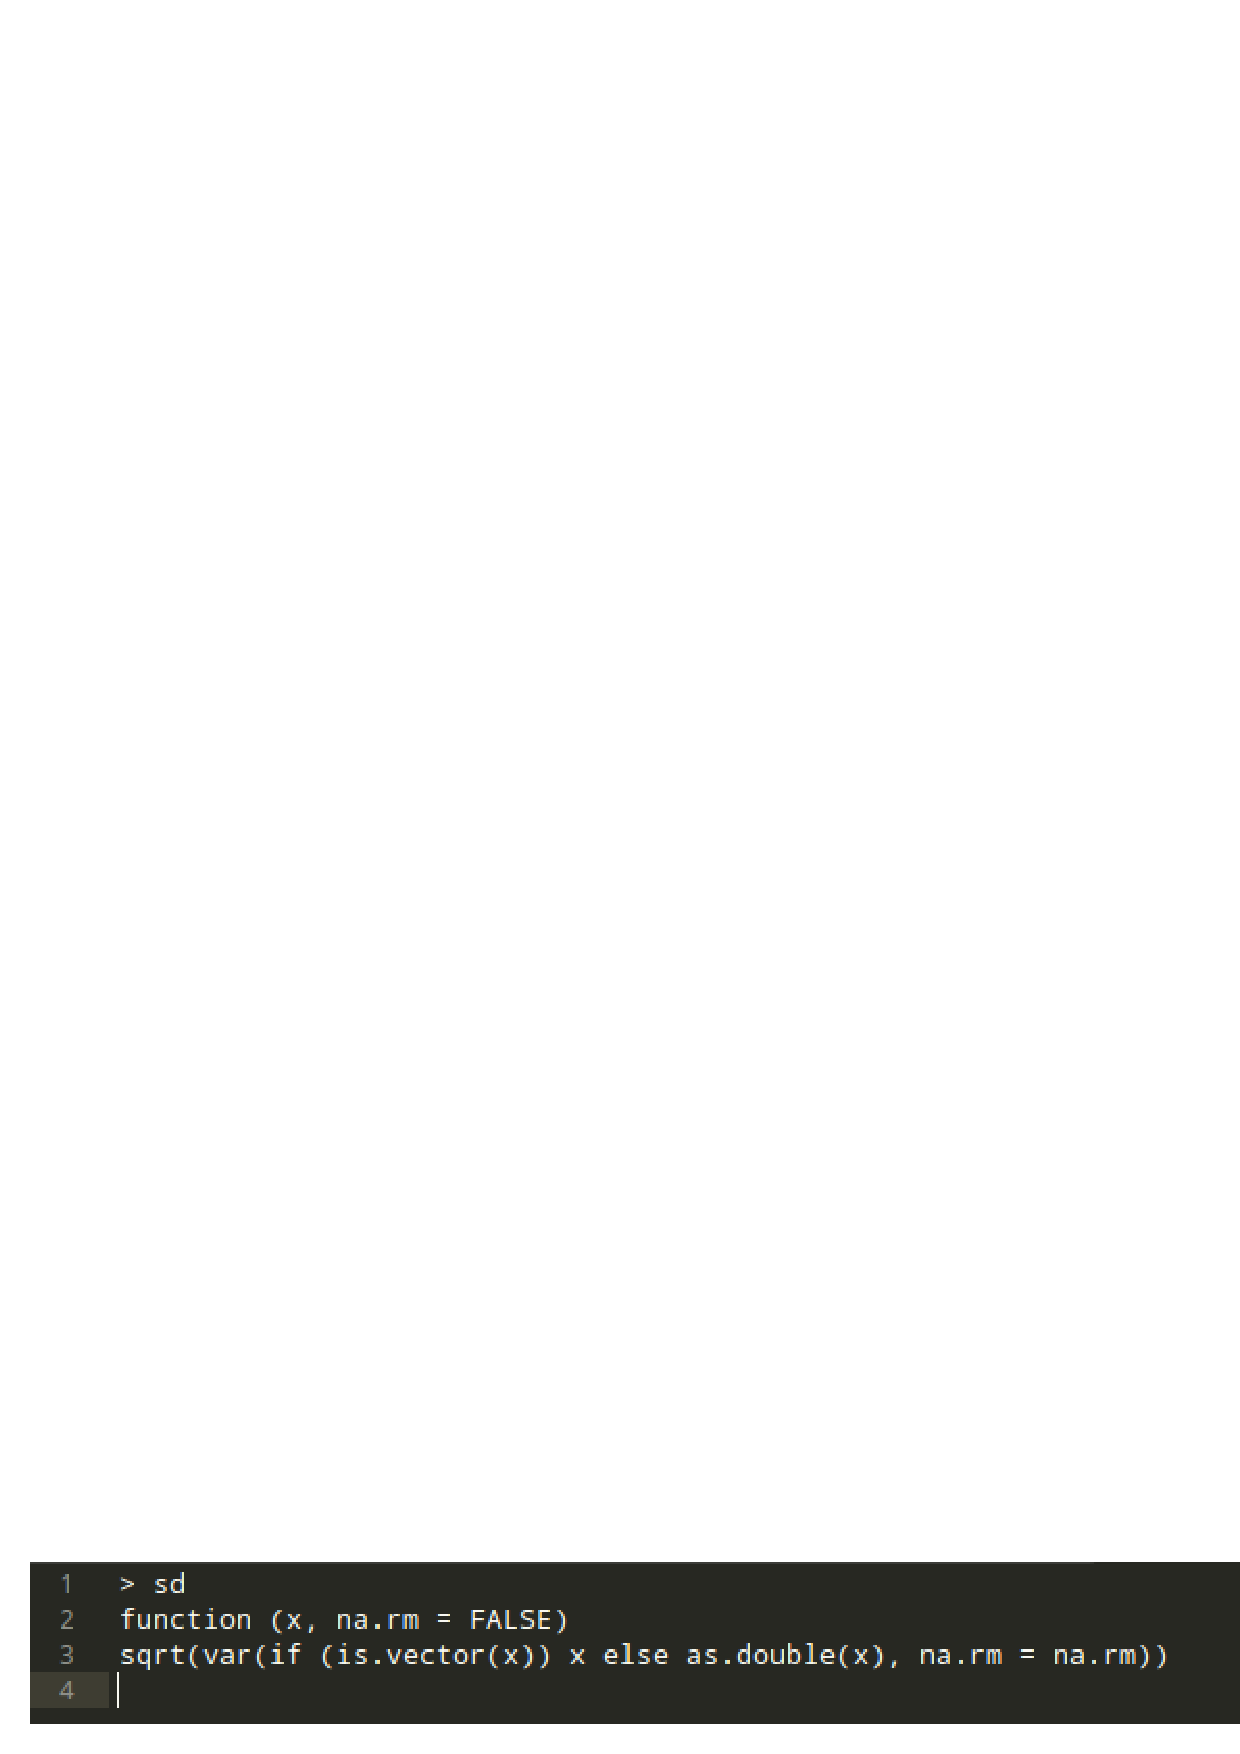
\includegraphics[width=90mm]{pictures/sd.jpg}
\label{overflow}
\end{figure}
\end{frame}


\begin{frame}[fragile]{factor}
\begin{figure}[ht!]
\centering
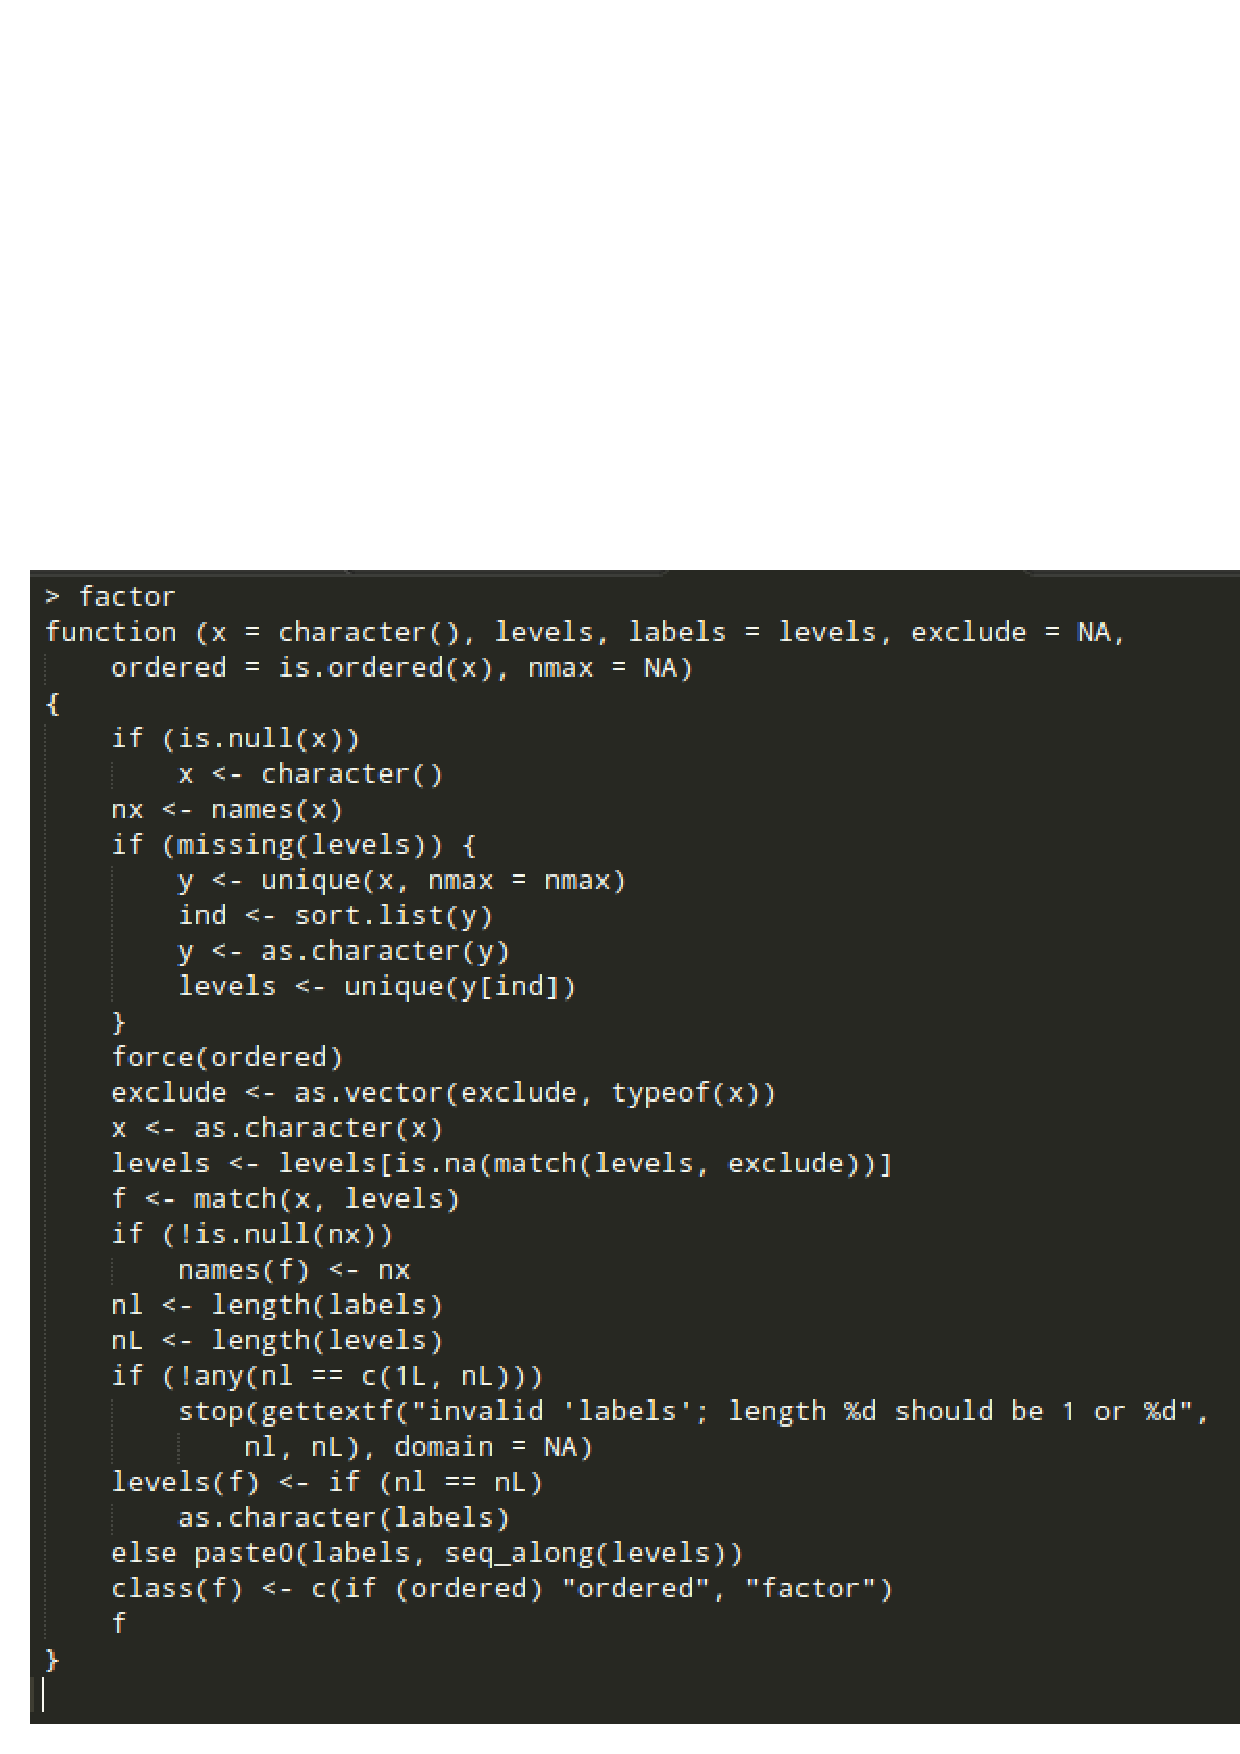
\includegraphics[width=90mm]{pictures/factor.jpg}
\label{overflow}
\end{figure}
\end{frame}


\begin{frame}[fragile]{table}
\begin{figure}[ht!]
\centering

\includegraphics[width=90mm]{pictures/table.jpg}
\label{overflow}
\end{figure}
\end{frame}


\begin{frame}[fragile]{Summary - why use functions?}

\begin{itemize}
\item Able to write general code to re-use
\item Free's up cognative space
\item Makes debugging easier
\item Easier to read - broken into logical blocks of code
\end{itemize}
Imagine having to write each function from scratch, or include it in your script every time you wanted to use it.
\linebreak
Just adding numbers using sum shows us how much we rely on functions.
\linebreak
\linebreak
Now that I have (hopefully) convinced you of why to use functions, here is a closer look at the syntax.
\end{frame}

\begin{frame}[fragile]{Syntax}
Lets take a closer look at the syntax...
\begin{knitrout}
\definecolor{shadecolor}{rgb}{0.969, 0.969, 0.969}\color{fgcolor}\begin{kframe}
\begin{alltt}
f <- \hlkwd{function}(<arguments>) \{
\hlcom{## Do something interesting}
\}
\end{alltt}
\end{kframe}
\end{knitrout}

And, with our example...
\begin{knitrout}
\definecolor{shadecolor}{rgb}{0.969, 0.969, 0.969}\color{fgcolor}\begin{kframe}
\begin{alltt}
\hlstd{calcBMI} \hlkwb{<-} \hlkwa{function}\hlstd{(}\hlkwc{weights}\hlstd{,} \hlkwc{heights}\hlstd{) \{}
    \hlstd{x} \hlkwb{<-} \hlstd{weights}\hlopt{/}\hlstd{(heights} \hlopt{*} \hlstd{heights)}
    \hlkwd{return}\hlstd{(x)}
\hlstd{\}}
\end{alltt}
\end{kframe}
\end{knitrout}

\end{frame}

\begin{frame}[fragile]{Syntax contd.}
Lets take a look at the inner workings of the function: mean
\begin{knitrout}
\definecolor{shadecolor}{rgb}{0.969, 0.969, 0.969}\color{fgcolor}\begin{kframe}
\begin{alltt}
\hlstd{mean.default}
\end{alltt}
\begin{verbatim}
## function (x, trim = 0, na.rm = FALSE, ...) 
## {
##     if (!is.numeric(x) && !is.complex(x) && !is.logical(x)) {
##         warning("argument is not numeric or logical: returning NA")
##         return(NA_real_)
##     }
##     if (na.rm) 
##         x <- x[!is.na(x)]
##     if (!is.numeric(trim) || length(trim) != 1L) 
##         stop("'trim' must be numeric of length one")
##     n <- length(x)
##     if (trim > 0 && n) {
##         if (is.complex(x)) 
##             stop("trimmed means are not defined for complex data")
##         if (anyNA(x)) 
##             return(NA_real_)
##         if (trim >= 0.5) 
##             return(stats::median(x, na.rm = FALSE))
##         lo <- floor(n * trim) + 1
##         hi <- n + 1 - lo
##         x <- sort.int(x, partial = unique(c(lo, hi)))[lo:hi]
##     }
##     .Internal(mean(x))
## }
## <bytecode: 0x2d40e88>
## <environment: namespace:base>
\end{verbatim}
\end{kframe}
\end{knitrout}

\end{frame}

% Now you have a grasp on the syntax of a function, lets try write our own.
\begin{frame}[fragile]{Writing our own!}
Lets write a function to calculate the average age of a group of rally drivers.
\begin{knitrout}
\definecolor{shadecolor}{rgb}{0.969, 0.969, 0.969}\color{fgcolor}\begin{kframe}
\begin{alltt}
\hlstd{ages} \hlkwb{<-} \hlkwd{c}\hlstd{(}\hlnum{27}\hlstd{,} \hlnum{24}\hlstd{,} \hlnum{35}\hlstd{,} \hlnum{24}\hlstd{,} \hlnum{24}\hlstd{,} \hlnum{33}\hlstd{,} \hlnum{35}\hlstd{,} \hlnum{22}\hlstd{,} \hlnum{28}\hlstd{)}

\hlstd{average} \hlkwb{<-} \hlkwa{function}\hlstd{(}\hlkwc{x}\hlstd{) \{}
    \hlstd{sumx} \hlkwb{<-} \hlkwd{sum}\hlstd{(x)}
    \hlstd{countx} \hlkwb{<-} \hlkwd{length}\hlstd{(x)}
    \hlkwd{return}\hlstd{(sumx}\hlopt{/}\hlstd{countx)}
\hlstd{\}}

\hlkwd{average}\hlstd{(ages)}
\end{alltt}
\begin{verbatim}
## [1] 28
\end{verbatim}
\end{kframe}
\end{knitrout}

\end{frame}


\begin{frame}[fragile]{Built in functions}
There are lots of built in functions!
\linebreak
We cheated a little in the above example, by making use of functions within our example function.
\linebreak
\linebreak
\begin{knitrout}
\definecolor{shadecolor}{rgb}{0.969, 0.969, 0.969}\color{fgcolor}\begin{kframe}
\begin{alltt}
\hlkwd{sum}\hlstd{()}
\end{alltt}
\end{kframe}
\end{knitrout}

is a function.
\linebreak
\linebreak
In fact, we could have just used the function:
\begin{knitrout}
\definecolor{shadecolor}{rgb}{0.969, 0.969, 0.969}\color{fgcolor}\begin{kframe}
\begin{alltt}
\hlkwd{mean}\hlstd{(ages)}
\end{alltt}
\begin{verbatim}
## [1] 28
\end{verbatim}
\end{kframe}
\end{knitrout}

\end{frame}

%\begin{frame}[fragile]{Environments}
%\begin{figure}[ht!]
%\centering
%\includegraphics[width=90mm]{pictures/environments.jpeg}
%\label{overflow}
%\end{figure}
%\end{frame}

\begin{frame}[fragile]{A word about environment}
Setting a variable
\begin{knitrout}
\definecolor{shadecolor}{rgb}{0.969, 0.969, 0.969}\color{fgcolor}\begin{kframe}
\begin{alltt}
\hlstd{var} \hlkwb{<-} \hlkwd{c}\hlstd{(}\hlnum{1}\hlstd{,} \hlnum{2}\hlstd{,} \hlnum{3}\hlstd{)}
\end{alltt}
\end{kframe}
\end{knitrout}

Seeing what is inside that variable.
\begin{knitrout}
\definecolor{shadecolor}{rgb}{0.969, 0.969, 0.969}\color{fgcolor}\begin{kframe}
\begin{alltt}
\hlkwd{print}\hlstd{(var)}
\end{alltt}
\begin{verbatim}
## [1] 1 2 3
\end{verbatim}
\end{kframe}
\end{knitrout}

\end{frame}
%Show how a variable set inside a function, is local to that function. demo error.
%Draw a picture

\begin{frame}[fragile]{Variables set inside functions, are local to functions}
Setting the variable inside a function
\begin{knitrout}
\definecolor{shadecolor}{rgb}{0.969, 0.969, 0.969}\color{fgcolor}\begin{kframe}
\begin{alltt}
\hlstd{create_var} \hlkwb{<-} \hlkwa{function}\hlstd{() \{}
    \hlstd{var2} \hlkwb{<-} \hlkwd{c}\hlstd{(}\hlnum{1}\hlstd{,} \hlnum{2}\hlstd{,} \hlnum{3}\hlstd{)}
\hlstd{\}}
\end{alltt}
\end{kframe}
\end{knitrout}

Call the function
\begin{knitrout}
\definecolor{shadecolor}{rgb}{0.969, 0.969, 0.969}\color{fgcolor}\begin{kframe}
\begin{alltt}
\hlkwd{create_var}\hlstd{()}
\end{alltt}
\end{kframe}
\end{knitrout}

Try see whats inside the variable.
\begin{knitrout}
\definecolor{shadecolor}{rgb}{0.969, 0.969, 0.969}\color{fgcolor}\begin{kframe}
\begin{alltt}
\hlkwd{print}\hlstd{(var2)}
\end{alltt}


{\ttfamily\noindent\bfseries\color{errorcolor}{\#\# Error: object 'var2' not found}}\end{kframe}
\end{knitrout}

\end{frame}

\begin{frame}[fragile]{Variables set outside functions, are globally available}
Setting the variable outside a function
\begin{knitrout}
\definecolor{shadecolor}{rgb}{0.969, 0.969, 0.969}\color{fgcolor}\begin{kframe}
\begin{alltt}
\hlstd{var3} \hlkwb{<-} \hlkwd{c}\hlstd{(}\hlnum{1}\hlstd{,} \hlnum{2}\hlstd{,} \hlnum{3}\hlstd{)}
\end{alltt}
\end{kframe}
\end{knitrout}

Make the function
\begin{knitrout}
\definecolor{shadecolor}{rgb}{0.969, 0.969, 0.969}\color{fgcolor}\begin{kframe}
\begin{alltt}
\hlstd{print_var} \hlkwb{<-} \hlkwa{function}\hlstd{() \{}
    \hlkwd{print}\hlstd{(var3)}
\hlstd{\}}
\end{alltt}
\end{kframe}
\end{knitrout}

Try see whats inside the variable, from within the function.
\linebreak
Call the function.
\begin{knitrout}
\definecolor{shadecolor}{rgb}{0.969, 0.969, 0.969}\color{fgcolor}\begin{kframe}
\begin{alltt}
\hlkwd{print_var}\hlstd{()}
\end{alltt}
\begin{verbatim}
## [1] 1 2 3
\end{verbatim}
\end{kframe}
\end{knitrout}

\end{frame}


\begin{frame}[fragile]{Environments contd.}
One last note on environments.
\begin{knitrout}
\definecolor{shadecolor}{rgb}{0.969, 0.969, 0.969}\color{fgcolor}\begin{kframe}
\begin{alltt}
\hlstd{df} \hlkwb{=} \hlkwd{data.frame}\hlstd{(}\hlkwc{col1} \hlstd{=} \hlnum{1}\hlopt{:}\hlnum{10}\hlstd{,} \hlkwc{col2} \hlstd{=} \hlkwd{rnorm}\hlstd{(}\hlnum{10}\hlstd{))}

\hlkwd{print}\hlstd{(df)}
\end{alltt}
\begin{verbatim}
##    col1    col2
## 1     1 -0.2004
## 2     2  1.1114
## 3     3  0.5627
## 4     4  1.2538
## 5     5  0.2058
## 6     6  1.8460
## 7     7  1.9196
## 8     8  1.0385
## 9     9  0.4043
## 10   10 -0.3654
\end{verbatim}
\end{kframe}
\end{knitrout}


\end{frame}

\begin{frame}[fragile]{Environments contd.}
Can we access those col1 and col2 variables?
\begin{knitrout}
\definecolor{shadecolor}{rgb}{0.969, 0.969, 0.969}\color{fgcolor}\begin{kframe}
\begin{alltt}
\hlkwd{print}\hlstd{(col1)}
\end{alltt}


{\ttfamily\noindent\bfseries\color{errorcolor}{\#\# Error: object 'col1' not found}}\end{kframe}
\end{knitrout}

Looks like not... 
\begin{knitrout}
\definecolor{shadecolor}{rgb}{0.969, 0.969, 0.969}\color{fgcolor}\begin{kframe}
\begin{alltt}
\hlstd{df} \hlkwb{<-} \hlkwd{transform}\hlstd{(df,} \hlkwc{col3} \hlstd{= col1} \hlopt{+} \hlstd{col2)}

\hlkwd{print}\hlstd{(df)}
\end{alltt}
\begin{verbatim}
##    col1    col2   col3
## 1     1 -0.2004 0.7996
## 2     2  1.1114 3.1114
## 3     3  0.5627 3.5627
## 4     4  1.2538 5.2538
## 5     5  0.2058 5.2058
## 6     6  1.8460 7.8460
## 7     7  1.9196 8.9196
## 8     8  1.0385 9.0385
## 9     9  0.4043 9.4043
## 10   10 -0.3654 9.6346
\end{verbatim}
\end{kframe}
\end{knitrout}

\end{frame}

\begin{frame}[fragile]{Environments contd.}
But thats really strange, how did it know what col1 and 2 were?
\linebreak
\linebreak
\pause
Because we gave it the variable 'myList', which has its own environmental variables.
\end{frame}



\begin{frame}[fragile]{Arguments}
Functions can be passed named arguments, or positional arguments.
\linebreak
Named arguments example:
\begin{knitrout}
\definecolor{shadecolor}{rgb}{0.969, 0.969, 0.969}\color{fgcolor}\begin{kframe}
\begin{alltt}
\hlstd{f} \hlkwb{<-} \hlkwa{function}\hlstd{(}\hlkwc{first}\hlstd{,} \hlkwc{second}\hlstd{) \{}
    \hlstd{x} \hlkwb{<-} \hlstd{first} \hlopt{-} \hlstd{second}
    \hlkwd{return}\hlstd{(x)}
\hlstd{\}}
\hlkwd{f}\hlstd{(}\hlkwc{first} \hlstd{=} \hlnum{10}\hlstd{,} \hlkwc{second} \hlstd{=} \hlnum{8}\hlstd{)}
\end{alltt}
\begin{verbatim}
## [1] 2
\end{verbatim}
\end{kframe}
\end{knitrout}

And we could equally do
\begin{knitrout}
\definecolor{shadecolor}{rgb}{0.969, 0.969, 0.969}\color{fgcolor}\begin{kframe}
\begin{alltt}
\hlkwd{f}\hlstd{(}\hlkwc{second} \hlstd{=} \hlnum{8}\hlstd{,} \hlkwc{first} \hlstd{=} \hlnum{10}\hlstd{)}
\end{alltt}
\begin{verbatim}
## [1] 2
\end{verbatim}
\end{kframe}
\end{knitrout}

Because these are named, the order in which we pass them to the function does not matter.
\end{frame}

\begin{frame}[fragile]{arguments contd.}
Positional
\linebreak
\begin{knitrout}
\definecolor{shadecolor}{rgb}{0.969, 0.969, 0.969}\color{fgcolor}\begin{kframe}
\begin{alltt}
\hlstd{f} \hlkwb{<-} \hlkwa{function}\hlstd{(}\hlkwc{first}\hlstd{,} \hlkwc{second}\hlstd{) \{}
    \hlstd{x} \hlkwb{<-} \hlstd{first} \hlopt{-} \hlstd{second}
    \hlkwd{return}\hlstd{(x)}
\hlstd{\}}
\end{alltt}
\end{kframe}
\end{knitrout}

Now if we swap the order, the results change
\begin{knitrout}
\definecolor{shadecolor}{rgb}{0.969, 0.969, 0.969}\color{fgcolor}\begin{kframe}
\begin{alltt}
\hlkwd{f}\hlstd{(}\hlnum{10}\hlstd{,} \hlnum{8}\hlstd{)}
\end{alltt}
\begin{verbatim}
## [1] 2
\end{verbatim}
\begin{alltt}
\hlkwd{f}\hlstd{(}\hlnum{8}\hlstd{,} \hlnum{10}\hlstd{)}
\end{alltt}
\begin{verbatim}
## [1] -2
\end{verbatim}
\end{kframe}
\end{knitrout}

\end{frame}

\begin{frame}[fragile]{So many ways to call a function}
This means that all of these are equivalent:
\begin{knitrout}
\definecolor{shadecolor}{rgb}{0.969, 0.969, 0.969}\color{fgcolor}\begin{kframe}
\begin{alltt}
\hlkwd{seq}\hlstd{(}\hlkwc{from} \hlstd{=} \hlnum{1}\hlstd{,} \hlkwc{to} \hlstd{=} \hlnum{10}\hlstd{,} \hlkwc{by} \hlstd{=} \hlnum{1}\hlstd{)}
\end{alltt}
\begin{verbatim}
##  [1]  1  2  3  4  5  6  7  8  9 10
\end{verbatim}
\begin{alltt}
\hlkwd{seq}\hlstd{(}\hlnum{1}\hlstd{,} \hlnum{10}\hlstd{,} \hlnum{1}\hlstd{)}
\end{alltt}
\begin{verbatim}
##  [1]  1  2  3  4  5  6  7  8  9 10
\end{verbatim}
\begin{alltt}
\hlkwd{seq}\hlstd{(}\hlkwc{by} \hlstd{=} \hlnum{1}\hlstd{,} \hlnum{1}\hlstd{,} \hlnum{10}\hlstd{)}
\end{alltt}
\begin{verbatim}
##  [1]  1  2  3  4  5  6  7  8  9 10
\end{verbatim}
\begin{alltt}
\hlkwd{seq}\hlstd{(}\hlkwc{to} \hlstd{=} \hlnum{10}\hlstd{,} \hlkwc{by} \hlstd{=} \hlnum{1}\hlstd{,} \hlkwc{from} \hlstd{=} \hlnum{1}\hlstd{)}
\end{alltt}
\begin{verbatim}
##  [1]  1  2  3  4  5  6  7  8  9 10
\end{verbatim}
\end{kframe}
\end{knitrout}

\end{frame}


\begin{frame}[fragile]{Missing and defaults}
Its possible to skip arguments, or assign defaults
\begin{knitrout}
\definecolor{shadecolor}{rgb}{0.969, 0.969, 0.969}\color{fgcolor}\begin{kframe}
\begin{alltt}
\hlstd{ages} \hlkwb{<-} \hlkwd{c}\hlstd{(}\hlnum{34}\hlstd{,} \hlnum{52}\hlstd{,} \hlnum{23}\hlstd{,} \hlnum{33}\hlstd{,} \hlnum{33}\hlstd{,} \hlnum{41}\hlstd{)}
\hlstd{f} \hlkwb{<-} \hlkwa{function}\hlstd{(}\hlkwc{a}\hlstd{,} \hlkwc{b}\hlstd{,} \hlkwc{c} \hlstd{=} \hlnum{TRUE}\hlstd{) \{}
    \hlkwd{print}\hlstd{(}\hlkwd{mean}\hlstd{(a))}
    \hlkwd{print}\hlstd{(c)}
\hlstd{\}}
\hlkwd{f}\hlstd{(ages)}
\end{alltt}
\begin{verbatim}
## [1] 36
## [1] TRUE
\end{verbatim}
\end{kframe}
\end{knitrout}

This works even without passing in b or c.
\end{frame}



\begin{frame}[fragile]{Partial matching}
When matching arguments, R will try and match part of a arguments name. This is know as Partial matching.
\begin{knitrout}
\definecolor{shadecolor}{rgb}{0.969, 0.969, 0.969}\color{fgcolor}\begin{kframe}
\begin{alltt}
\hlstd{f} \hlkwb{<-} \hlkwa{function}\hlstd{(}\hlkwc{first}\hlstd{,} \hlkwc{second}\hlstd{) \{}
    \hlkwd{print}\hlstd{(first)}
    \hlkwd{print}\hlstd{(second)}
\hlstd{\}}
\hlkwd{f}\hlstd{(}\hlkwc{first} \hlstd{=} \hlstr{"first argument"}\hlstd{,} \hlkwc{sec} \hlstd{=} \hlstr{"second argument"}\hlstd{)}
\end{alltt}
\begin{verbatim}
## [1] "first argument"
## [1] "second argument"
\end{verbatim}
\end{kframe}
\end{knitrout}

We only partly name "second" as "sec". And R still understands.
\end{frame}

\begin{frame}[fragile]{Order of matching}
\linebreak
When trying to match arguments, R will test in the following order:
\linebreak
1) exact match.
\linebreak
2) partial match.
\linebreak
3) positional match
\end{frame}

\begin{frame}[fragile]{}
You might also see "...".
\linebreak
This just means, a variable number of arguments. Typically, they are passed onto other functions.
\end{frame}

\begin{frame}[fragile]{Return}
We can pass arguments to a function, and functions are able to return values to where they were called.
\begin{knitrout}
\definecolor{shadecolor}{rgb}{0.969, 0.969, 0.969}\color{fgcolor}\begin{kframe}
\begin{alltt}
\hlstd{f} \hlkwb{<-} \hlkwa{function}\hlstd{() \{}
    \hlkwd{return}\hlstd{(}\hlnum{10}\hlstd{)}
\hlstd{\}}
\hlkwd{f}\hlstd{()}
\end{alltt}
\begin{verbatim}
## [1] 10
\end{verbatim}
\end{kframe}
\end{knitrout}

We are able to capture this return value.
\begin{knitrout}
\definecolor{shadecolor}{rgb}{0.969, 0.969, 0.969}\color{fgcolor}\begin{kframe}
\begin{alltt}
\hlstd{x} \hlkwb{<-} \hlkwd{f}\hlstd{()}
\hlkwd{print}\hlstd{(x)}
\end{alltt}
\begin{verbatim}
## [1] 10
\end{verbatim}
\end{kframe}
\end{knitrout}

\end{frame}

\begin{frame}[fragile]{Return}
Some functions return lots.
\begin{knitrout}
\definecolor{shadecolor}{rgb}{0.969, 0.969, 0.969}\color{fgcolor}\begin{kframe}
\begin{alltt}
\hlstd{year} \hlkwb{<-} \hlkwd{c}\hlstd{(}\hlnum{2000}\hlstd{,} \hlnum{2001}\hlstd{,} \hlnum{2002}\hlstd{,} \hlnum{2003}\hlstd{,} \hlnum{2004}\hlstd{)}
\hlstd{rate} \hlkwb{<-} \hlkwd{c}\hlstd{(}\hlnum{9.34}\hlstd{,} \hlnum{8.5}\hlstd{,} \hlnum{7.62}\hlstd{,} \hlnum{6.93}\hlstd{,} \hlnum{6.6}\hlstd{)}
\hlstd{fit} \hlkwb{<-} \hlkwd{lm}\hlstd{(rate} \hlopt{~} \hlstd{year)}
\hlkwd{attributes}\hlstd{(fit)}
\end{alltt}
\begin{verbatim}
## $names
##  [1] "coefficients"  "residuals"     "effects"       "rank"         
##  [5] "fitted.values" "assign"        "qr"            "df.residual"  
##  [9] "xlevels"       "call"          "terms"         "model"        
## 
## $class
## [1] "lm"
\end{verbatim}
\begin{alltt}
\hlstd{fit}\hlopt{$}\hlstd{residuals}
\end{alltt}
\begin{verbatim}
##      1      2      3      4      5 
##  0.132 -0.003 -0.178 -0.163  0.212
\end{verbatim}
\end{kframe}
\end{knitrout}

\end{frame}


\begin{frame}[fragile]{Summary}
We should now understand:
\begin{itemize}
\item What a library is, and where they are.
\item What a package is, and how to get more.
\item How to load a package for use.
\item What a script is.
\item What a function is, and how to write your own.
\item Why functions are useful.
\item What arguments are, and different ways to pass them.
\item What an environment is, the difference between local and global.
\item Returning values from functions.
\end{itemize}
\end{frame}

\begin{frame}[fragile]{end}
Thank you.
\end{frame}

\begin{frame}[fragile]{Tutorial}



\begin{itemize}
\item Describe the heirachy of packages, functions and libraries.
\item List the libraries on your computer.
\item Give 5 packges that are already installed on your machine.
\item Find and install the "Xtable" package from CRAN.
\item Load any package into your R environment, and make use of some piece of it, without errors.
\item Write your own function to take two numbers, multiply them, and print the result within the function.
\item Make sure your function can accept arguments by name.
\item Call your function using partial matching.
\end{itemize}
\end{frame}


\end{document}
